% !TEX root = main.tex
\chapter{Flavour Tagging}
\label{ch:flavourtagging}

To measure interference \CP-violation the production flavour of $B$-mesons under study must be known.
At \lhcb this is inferred using the so-called flavour tagging.
The flavour tagging algorithms (taggers) provide for each candidate both, a decision (tag) $d$ whether it initiallly was a \Bz-meson or a \Bzb-meson and a probability-estimate (mistag) $\eta$ of being wrong with this decision.
They can be divided into two classes: Opposite side (OS) and same side (SS) algorithms.
In this chapter first a general description of the different algorithms available at \lhcb, their performance characteristics and their calibration is given (\cref{sec:taggingalgorithms}).
Following, the tagging strategy for this analysis is outlined in \cref{sec:taggingstrategy} and the calibration of the OS tagging algorithms is summarised (\cref{sec:OScalibration}).
Last the required retraining and the calibration of the SS tagging algorithms presented (\cref{sec:SScalibration}).

\section{Tagging algorithms}
\label{sec:taggingalgorithms}

At \lhcb several tagging algorithms exist to infer the initial $B$ flavour which slightly differ for \Bz and \Bs mesons.
In \cref{fig:taggingalgorithms} a schematic representation of the tagging algorithms for \Bz mesons is shown.
\begin{figure}[tbp]
    \centering
    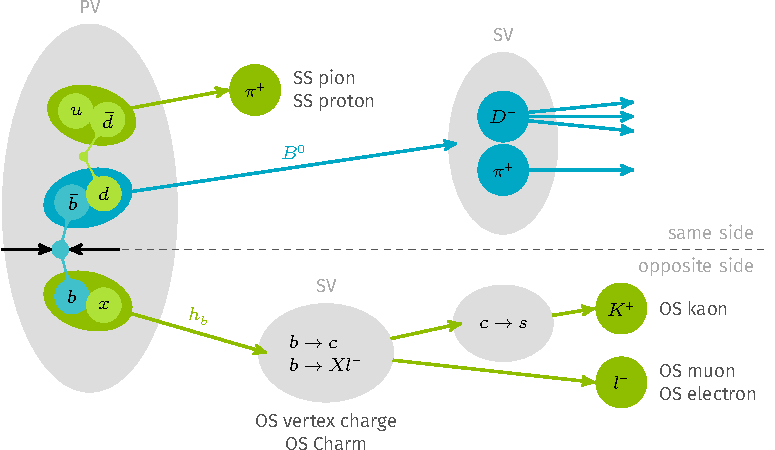
\includegraphics[width=0.8\textwidth]{08FlavourTagging/figs/FTscheme.pdf}
    \caption{Schematic overview of all available \Bz tagging algorithms.}
    \label{fig:taggingalgorithms}
\end{figure}
They can be separated into so-called opposite side (OS) and same side (SS) algorithms.

The OS algorithms exploit the production and decay of the second \bquark-quark which is produced in the proton-proton collision.
By partially reconstructing single decay products as electrons, muons, kaons and \D-mesons associated with the decay of the opposite side \bquark-hadron the initial flavour is inferred.
Furthermore charged tracks which originate from a secondary vertex which is displaced from the \ac{PV} are used to make a decision on the production flavour of the signal $B$-meson.
As the hadronisation and the decay of the OS \bquark-hadron is independent of the signal \bquark-quark these algorithms can be used for both \Bz and \Bs mesons. Based on \cite{LHCb-PAPER-2011-027, LHCb-PAPER-2015-027} the OS algorithms are shortly described in the following:
\begin{itemize}
	\item The OS muon and OS electron tagger use the charge of muons and electrons from semileptonic $\bquark\!\to Xl^-$ decays to take a decision on the initial $B$-flavour.
	The charged leptons are selected using a simple cut-based selection.
	To suppress contributions from $\bquark\!\to\cquark\!\to l^+$ decays, which would give the wrong tag decision the transverse momentum of the muon (electron) is required to be larger than \SI[per-mode=symbol]{1.2}{\GeVc} (\SI[per-mode=symbol]{1.0}{\GeVc}) for example.
	Electrons have additionally to satisfy criteria on electron identification variables such as the ratio $\nicefrac{E}{p}>0.8$.
	Here $E$ denotes the energy deposited in the ECAL and $p$ the electron momentum.
	If more than one lepton per event survives the selcection the lepton with highest transverse momentum is chosen to define the flavour of the signal $B$.
	The mistag is estimated with an artificial neural-network, which takes as inputs event properties as the number of \ac{PV}s and tracks in the event, $B$-properties as the transverse momentum, and various geometrical and kinematic properties of the lepton.
	\item The OS kaon tagger explores the charge of kaons produced in the decay chain $\bquark\!\to\cquark\!\to\squark$.
	Very similar to the lepton taggers the tagging kaon is selected using a cut-based selection based on kinematic and PID observables.
	In case multiple kaons per event pass this selection, the kaon with highest transverse momentum is fed into an artificial neural network with similar inputs as for the lepton taggers to calculate the mistag estimate $\eta$.
	\item The OS charm tagger selects \D-mesons produced via $\bquark\!\to\cquark$ decays.
	In case of a charged \D-meson the charge of the meson directly hints at the initial flavour, in case of an uncharged \D-meson the charge of the produced kaon is used to infer the flavour of the signal $B$-meson.
	In contrast to the other single track taggers a \ac{BDT} is used to select the \D-meson and estimate the mistag.
	As the OS charm is the newest development on the OS it was developed to have a small overlap concerning the used tagging particles with the other taggers.
	\item The OS vertex charge tagger is the only algorithm which does note reconstruct a single particle, but instead uses the weighted charge of a \ac{SV} associated with the opposite side \bquark-hadron.
	In order to to this, the track pair with the highest probability of originating from the opposite side \bquark-hadron is used to build a vertex.
	Particles which are compatible with coming from this two-track vertex but not from the \ac{PV} are are added to form the final \ac{SV}.
	Finally all tracks of this vertex are weighted with their transverse momentum, \pt, and used to calculate a charge
	\begin{equation}
	Q_{\text{vtx}}=\frac{\sum_{i}p_{\mathrm T}^k(i)Q_i}{\sum_{i}p_{\mathrm T}^k(i)}.
	\end{equation}
	where the parameter $k$ is optimised to maximise the performance of the tagging algorithm.
	From this charge then the initial flavour of the signal $B$-meson is derived.
\end{itemize}

The SS algorithms use remnants of the signal $B$ hadronisation to infer the initial flavour.
However, as the companion quark of the \bquark-quark differs between \Bz and \Bs mesons different same side taggers exist for these mesons.
In case of a \Bz (\bquarkbar\dquark) a free \dquarkbar is produced which can hadronise to a pion or proton.
On the other hand a \Bs (\bquarkbar\squark) leads to a \squarkbar which can hadronise to a kaon.




\subsection{Performance characteristics}

\subsection{Tagging calibration}

\section{Flavour tagging strategy}
\label{sec:taggingstrategy}


\section{Opposite side tagging calibration}
\label{sec:OScalibration}


\section{Same side tagging calibration}
\label{sec:SScalibration}

\subsection[head={Selection and mass fit of $\Bz\!\to\jpsi\Kstarz$ candidates},tocentry={Selection and mass fit of $\Bz\!\to\jpsi\Kstarz$ candidates}]{Selection and mass fit of $\symbfsf{\Bz\!\to\jpsi\Kstarz}$ candidates}


\subsection{Retraining of the SS pion tagger}


\subsection{Retraining of the SS proton tagger}


\subsection{Calibration portability}
